\documentclass[10pt,a4paper]{article}
\usepackage[utf8]{inputenc}
\usepackage{amsmath}
\usepackage{amsfonts}
\usepackage{amssymb}
\usepackage{graphicx}
\usepackage{subfigure}
\usepackage{amsmath}
\usepackage{mathrsfs}
\DeclareRobustCommand{\orderof}{\ensuremath{\mathcal{O}}}
\bibliographystyle{prsty}
\usepackage[top=1in, bottom=1in, left=1in, right=1in]{geometry}

\begin{document}
\section{Introduction}
\textbf{flq\_ban} is a task of extension level. It calculates the Floquet band structure. To use this task, you must first perform \textbf{flq} first. All of the keywords are the same with \textbf{ban}, so one should reference \textbf{ban} for details. Also, the attached output data are not complete because they are too large. Only the variable names are attached.  

\section{Dictionary}

\subsection{Input}
 \textbf{flq\_ban} shares exactly the same keywords as \textbf{ban}. Therefore, one can directly reference the dictionary of \textbf{ban}

\subsection{Output}
 \textbf{flq\_ban} shares exactly the same keywords as \textbf{ban}. Therefore, one can directly reference the dictionary of \textbf{ban} \\ \\
 \\ \\
 \\ \\
 \\ \\
 \\ \\
  \\ \\
  \\ \\
 \\ \\
 \\ \\
 \\ \\
 \\ \\
  \\ \\
  \\ \\
  \\ \\
  \\ 
  
  
\begin{figure}[tbp]
\centering
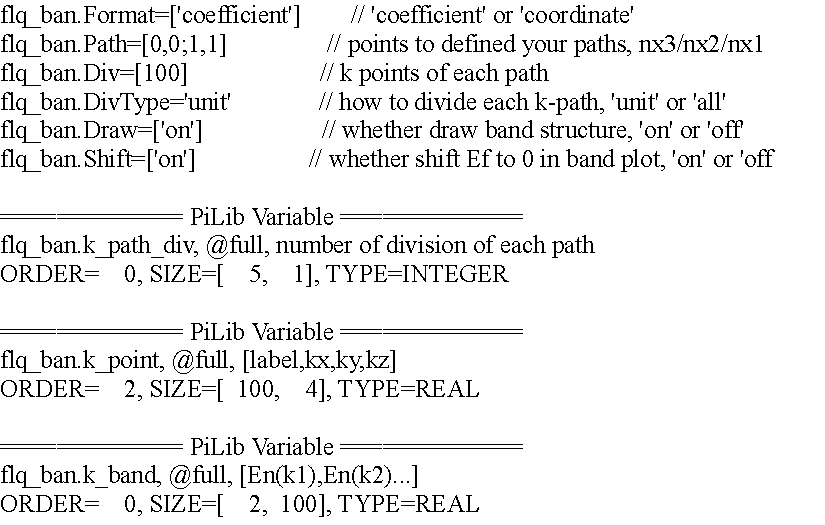
\includegraphics[width=0.9\columnwidth]{Haldane_flq_ban.pdf}
\caption{page 1 of Haldane\_flq\_ban.plb}
\end{figure}

\end{document}